\documentclass{CSUniSchoolLabReport}

\usepackage[italian]{babel}
\usepackage{fancyhdr}
\usepackage{xcolor,colortbl}
\usepackage[hidelinks]{hyperref}

\hypersetup{linktoc=all}
\graphicspath{ {./images/} }
\definecolor{lightgreen}{rgb}{0.75, 0.95, 0.75}
\definecolor{green}{rgb}{0.5, 0.85, 0.5}

\title{GreenTrails - Modulo AI}
\author{\textsc{Roberta Galluzzo}, \textsc{Gabriele Di Stefano}}

\pagestyle{fancy}
\renewcommand{\headrulewidth}{0pt}
\fancyhf{}
\lfoot{
\includegraphics[scale=0.05]{logo}
		GreenTrails - Modulo AI}
\rfoot{\thepage}

\begin{document}
\maketitle

\begin{center}
	
\includegraphics[scale=0.2]{logo}
\end{center}

\begin{center}
	\begin{tabular}{l r}
		Team: & C03 GreenTrails \\
		Progetto: & Progetto combinato IS/FIA 2023-2024 \\
		Repository: & \href{https://github.com/gab-ds/fia}{https://github.com/gab-ds/fia}
	\end{tabular}
\end{center}

\pagebreak

\tableofcontents

\pagebreak

\section{Definizione del problema}
\subsection{Introduzione}

Negli ultimi anni, l'ecosostenibilità è diventata una priorità, poiché il mondo, in rapida crescita, deve prestare maggiore attenzione all'ambiente. In questo contesto, l'applicazione web "GreenTrails" si rivolge al settore turistico, con l'obiettivo di facilitare l'organizzazione di viaggi sostenibili, tenendo conto delle sfide che gli utenti affrontano in questo ambito.
L'obiettivo di "GreenTrails" è permettere agli utenti di pianificare facilmente e rapidamente viaggi ecosostenibili, aiutandoli a individuare mete, strutture e attività adatte. \\\\
L'applicazione, dunque, mira a:
\begin{itemize}
    \item Facilitare la ricerca di strutture eco-friendly;
    \item Generare automaticamente itinerari in base alle preferenze personali degli utenti;
    \item Velocizzare il contatto con le strutture selezionate.
\end{itemize}

\pagebreak{}

\subsection{Obiettivi}

GreenTrails prevede, appunto, la \textbf{generazione automatica di itinerari multi-attività in base alle preferenze specificate dall'utente}, attraverso l'utilizzo di un algoritmo di intelligenza artificiale. Le preferenze sono così composte:
\begin{itemize}
    \item \textbf{Località preferita}: una scelta tra \textit{Mare}, \textit{Montagna}, \textit{Città}, oppure \textit{Nessuna preferenza}.
    \item \textbf{Tipologia di alloggio preferita}: uno tra \textit{Hotel}, \textit{Bed \& Breakfast}, \textit{Villaggio turistico}, \textit{Ostello} oppure \textit{Nessuna preferenza}.
    \item \textbf{Preferenze alimentari}: \textit{Vegan}, \textit{Vegetarian}, \textit{Gluten-free} o \textit{Nessuna preferenza}.
    \item \textbf{Tipologia di attività preferita}: una categoria a scelta tra \textit{All'aperto}, \textit{Visite storico-culturali}, \textit{Gastronomia} oppure \textit{Nessuna preferenza}.
    \item \textbf{Animale domestico}: esprime la preferenza di portare con sé un animale da compagnia, con una semplice scelta tra \textit{Sì} oppure \textit{No}.
    \item \textbf{Budget}: \textit{Basso}, \textit{Medio}, \textit{Alto} oppure \textit{Flessibile}.
    \item \textbf{Souvenir locali}: esprime l'interesse nell'acquisto di prodotti artigianali locali, con una semplice scelta tra \textit{Sì} oppure \textit{No}.
    \item \textbf{Stagione preferita}: \textit{Autunno-inverno}, \textit{Primavera-estate} o \textit{Nessuna preferenza}.
\end{itemize}
~\\
Inoltre, tale algoritmo dovrà rispettare il vincolo di dover generare un percorso valido entro il tempo massimo prestabilito dal sistema (\textbf{2 secondi}, come definito dal System Design Goal \textit{"DG\_12 - Tempo di risposta"}).


\subsubsection{Ulteriori considerazioni}

In mancanza di ulteriori specifiche, che avrebbero potuto maggiormente impostare il problema, si è deciso di imporre dei vincoli aggiuntivi per facilitare la fase di formulazione:
\begin{itemize}
	\item il modulo di intelligenza artificiale non cercherà su tutto il database dell'applicazione, ma soltanto su un subset fornito dal sistema stesso (in altre parole, \textbf{consideriamo soltanto le attività di una città o una specifica area} fornite dal sistema);
	\item il percorso dovrà \textbf{terminare con una e una sola struttura ricettiva};
	\item il percorso dovrà \textbf{contenere almeno due attività turistiche, fino ad un massimo di quattro};
	\item il percorso deve avere una \textbf{lunghezza massima di 5 km}.
    \item le attività del percorso \textbf{non possono essere ripetute}.
\end{itemize}

\pagebreak

\subsection{Specifica PEAS}

\begin{itemize}
 \item \textbf{Performance}: la misura di prestazione dell'agente, in questo caso, si basa sulla pertinenza del percorso fornito con le preferenze dell'utente e sulla sua distanza massima tra le attività.
 \item \textbf{Environment}: l'ambiente di riferimento è l'applicazione web di GreenTrails, la quale comunica direttamente con l'agente.
 \item \textbf{Actuators}: sono le soluzioni restituite all'applicazione web.
 \item \textbf{Sensors}: sono i dati in input (ovvero, la lista delle attività disponibili e le preferenze dell'utente) forniti dall'applicazione web.
\end{itemize}


\subsection{Caratteristiche dell'ambiente}

L'ambiente in cui opera l'agente ha le seguenti caratteristiche:
\begin{itemize}
 \item è \textbf{completamente osservabile}, in quanto prende in considerazione tutte le possibili attività fornite dal sistema;
 \item è \textbf{stocastico}, poiché lo stato varia indipendentemente dalle azioni dell'agente;
 \item è \textbf{episodico}, dal momento che la soluzione scelta dall'agente varia in base alla lista di attività e alle preferenze dell'utente (dunque, ad ogni episodio);
 \item è \textbf{statico}, in quanto non subisce variazioni mentre l'agente sta valutando le possibili soluzioni;
 \item è \textbf{discreto}, perché è possibile identificare un numero finito di scelte (tutte le possibili combinazioni di attività e strutture ricettive);
 \item è \textbf{ad agente singolo}, dato che consente la presenza di un unico agente.
\end{itemize}

\pagebreak

\subsection{Analisi del problema}

Considerando la natura del problema, che è di \textbf{ottimizzazione}, possiamo optare per l'utilizzo di un \textbf{algoritmo genetico}. Tale scelta è condizionata anche dalla \textbf{necessità progettuale} (per il progetto di Ingegneria del Software) di utilizzare un algoritmo genetico per la generazione degli itinerari. \\
Formalizzando:
\begin{itemize}
    \item \textbf{Spazio degli stati}: tutte le possibili permutazioni delle attività contenenti almeno due attività turistiche ed esattamente una struttura ricettiva al termine, con distanza massima complessiva di 5 km;
    \item \textbf{Stato iniziale}: percorso vuoto;
    \item \textbf{Azioni}: aggiungere un'attività turistica (fino ad un massimo di 4), o una struttura ricettiva (se è al termine del percorso);
    \item \textbf{Modello di transizione}: restituisce un percorso contenente l'attività aggiunta alla fine dello stesso;
    \item \textbf{Test obiettivo}: il percorso deve contenere attività basate sulle preferenze utente, e deve essere realizzato entro 2 secondi;
    \item \textbf{Costo di cammino}: distanza dall'attività successiva, in km.
\end{itemize}

\pagebreak{}
\section{Soluzione del problema}
\subsection{Set di dati utilizzati}

Per ciò che concerne il reperimento dei dati, sono disponibili due opzioni:

\begin{itemize}
    \item la prima, che consiste nell'\textbf{utilizzare un dataset pubblicamente disponibile};
    \item la seconda, che consiste nella \textbf{generazione di dati artificiali}.
\end{itemize}

Abbiamo optato per la generazione di dati artificiali, in quanto è irrilevante avere dati veritieri in questo contesto: \textbf{il focus del problema è quello di trovare dei percorsi affini in base alle esigenze dell'utente}, ed è perciò non necessario utilizzare informazioni di strutture e utenti reali. \\
Ci siamo avvalsi di \textit{due script aggiuntivi} per la generazione casuale dei dataset di visitatori e attività.

\subsubsection{Formattazione dei dati}

I dati sono stati organizzati in file con formato CSV, in modo da renderli facilmente leggibili e interpretabili sia da un software, sia da una persona che li esamini manualmente.

Ecco la composizione del set di dati dei visitatori, con una riga di esempio: \\

\begin{center}
\begin{tabular}{|c|c|} \hline\rowcolor{lightgreen}
\textbf{ID}                              & 1                        \\\rowcolor{green}
\textbf{Località preferita}              & Città                    \\\rowcolor{lightgreen}
\textbf{Tipologia di alloggio preferita} & Villaggio turistico      \\\rowcolor{green}
\textbf{Preferenze alimentari}           & Vegetarian               \\\rowcolor{lightgreen}
\textbf{Tipologia di attività preferita} & Visite storico-culturali \\\rowcolor{green}
\textbf{Animali domestici}               & Sì                       \\\rowcolor{lightgreen}
\textbf{Budget}                          & Medio                    \\\rowcolor{green}
\textbf{Souvenir locali}                 & Sì                       \\\rowcolor{lightgreen}
\textbf{Stagione preferita}              & Primavera-estate         \\\hline
\end{tabular}
\end{center}

Ecco la composizione del set di dati delle attività, con una riga di esempio: \\

\begin{center}
\begin{tabular}{|c|c|} \hline\rowcolor{lightgreen}
\textbf{ID}                 & 1                    \\\rowcolor{green}
\textbf{Latitudine}         & 45.66591297292027    \\\rowcolor{lightgreen}
\textbf{Longitudine}        & 10.475487956720567   \\\rowcolor{green}
\textbf{Alloggio}           & Sì                   \\\rowcolor{lightgreen}
\textbf{Tipologia}          & Villaggio turistico  \\\rowcolor{green}
\textbf{Prezzo}             & 478                  \\\rowcolor{lightgreen}
\textbf{Cibo}               & Vegan                \\\rowcolor{green}
\textbf{Animali domestici}  & Sì                   \\\rowcolor{lightgreen}
\textbf{Stagione rilevante} & Nessuna informazione \\\rowcolor{green}
\textbf{Souvenir locali}    & Sì                   \\\rowcolor{lightgreen}
\textbf{Località}           & Montagna			   \\\hline
\end{tabular}
\end{center}

\subsection{Tecnologie utilizzate}

Come linguaggio di programmazione, si è scelto di utilizzare \textbf{Python 3}.
Le librerie utilizzate, invece, sono molteplici; di seguito, quelle utilizzate dal programma agente:

\begin{itemize}
	\item \textbf{FastAPI}, per la realizzazione di un'API HTTP attraverso cui interagire con il sistema;
	\item \textbf{GeoPy}, per il corretto calcolo delle distanze geografiche;
	\item \textbf{SciPy}, per poter raggruppare i punti in un K-D Tree;
	\item \textbf{NumPy}, per velocizzare i calcoli, piuttosto che utilizzare le funzioni built-in di Python.
\end{itemize}

$ $\\
Ulteriori librerie utilizzate, che non fanno direttamente parte dell'agente, sono:
\begin{itemize}
	\item \textbf{PyCristoforo}, utilizzato per la corretta generazione di coordinate casuali in Italia, da utilizzare nel set di dati delle attività;
	\item \textbf{Requests}, utilizzato per lo script di mock del sistema che dovrà interagire con l'endpoint HTTP esposto dall'agente;
	\item \textbf{Pandas}, utilizzato per lo script di mock del sistema per caricare i dati dai rispettivi dataset di attività e visitatori;
	\item \textbf{Matplotlib}, utilizzato per la generazione dei grafici.
\end{itemize}

\pagebreak{}
\subsection{Specifica dell'algoritmo genetico}

\subsubsection{Codifica degli individui}

La nostra decisione è stata quella di determinare ogni individuo come un array a taglia fissa, di dimensione 5, contenente gli ID numerici delle attività, in cui l'ultimo elemento è sempre una struttura ricettiva. Per rappresentare eventuali percorsi con un numero di attività turistiche inferiori a 4, si è inoltre deciso di utilizzare un valore sentinella al posto dell'ID, con valore 0.

\subsubsection{Funzione di fitness}

La funzione di fitness \textit{f(x)} è così definita:

$$f(x) = w_{distanza} * \sum_{i=1}^{n-1} f_{distanza}(x_i, x_{i+1}) + w_{attivita} * \sum_{i=1}^{n} f_{attivita}(x_i) + w_{presente} * \sum_{i=1}^m presente(x_i)$$

I suoi componenti sono:
\begin{itemize}
    \item $w_{distanza}$: il peso della distanza nel fitness totale dell'individuo;
    \item $f_{distanza}$: il valore di fitness dipendente dalla distanza tra due punti, calcolato sottraendo a 5000 la distanza in metri ($5000 - distanza(x, y)$) e troncando il risultato ad un intero. Restituisce valore 0 se troppo distanti tra loro;
    \item $n$: è il numero di elementi (nel nostro caso, 5) che compongono ogni individuo;
    \item $w_{attivita}$: il peso della corrispondenza delle preferenze nel fitness totale;
    \item $f_{attivita}$: il valore di fitness dipendente dalla corrispondenza tra le preferenze utente e l'attività, dando un valore di reward di 2 per ogni corrispondenza perfetta (o nessuna preferenza espressa). Casi particolari sono la preferenza di stagione (nel caso in cui la struttura non abbia una stagione rilevante, ma l'utente abbia espresso una preferenza, la reward è dimezzata ad 1) e il budget (nel caso in cui non ci sia una corrispondenza perfetta, la reward sarà compresa tra -4 e +4, in base alla differenza tra budget preferito e prezzo effettivo). Restituisce la somma di tutte le reward;
    \item $w_{presente}$: il peso della presenza delle prime $m$ attività nel percorso;
    \item $presente(x_i)$: restituisce 1 se l'attività non è vuota, 0 altrimenti;
    \item $m$: è il numero degli elementi presi in considerazione per la reward di presenza (nel nostro caso, 2).
\end{itemize}
~\\
La reward di presenza è stata aggiunta in seguito, in modo da \textbf{valorizzare percorsi contenenti più attività}: senza di essa, l'algoritmo tenderebbe a privilegiare soluzioni di lunghezza minore, a scapito della completezza del percorso, portando a itinerari con al più 3 attività.\\
La funzione di fitness \textbf{restituisce valore 0 nel caso in cui i vincoli non siano rispettati} (attività troppo distanti o ripetute, permutazioni non accettabili).

\pagebreak{}

\subsubsection{Inizializzazione}

Per generare una popolazione iniziale con soluzioni accettabili, si è pensato di utilizzare il seguente algoritmo:

\texttt{1. Separa l'array delle attività in un array di sole strutture ricettive e un array di sole attività turistiche. \\
2. Costruisci due K-D Tree, uno contenente le coordinate delle sole attività turistiche, l'altro delle sole strutture ricettive. \\
3. Poni la distanza totale del percorso a 0. \\
4. Prendi casualmente una struttura ricettiva. \\
5. Estrai dal K-D Tree delle attività turistiche al massimo 5 attività più vicine all'attività di riferimento. \\
6. Scarta le attività turistiche che distano più di 5 km dall'attività di riferimento, escludendo anche le attività già presenti nell'individuo, lasciando soltanto quelle ammissibili. \\
7a. Se il numero di attività turistiche ammissibili è inferiore a 2, scarta la struttura ricettiva e torna al punto 3. \\
7b. Altrimenti, seleziona la prima attività più vicina, aggiungendo alla distanza totale la distanza tra le due attività. \\
8a. Se la distanza totale supera i 5 km, e le attività presenti finora nell'individuo sono almeno 3, aggiungi l'individuo alla popolazione e vai al punto 10. \\
8b. Altrimenti, se il loro numero non supera i 2 elementi, scarta la struttura ricettiva e torna al punto 3. \\
9. Ritorna al punto 4, utilizzando però l'ultima attività aggiunta come riferimento, finché non abbiamo al più 5 elementi nell'individuo. Se l'individuo ha esattamente 5 elementi, allora aggiungilo alla popolazione.
10. Ritorna al punto 3 finché il numero di individui è minore di n. 
}

Nell'algoritmo sopra specificato, si consideri $n$ la dimensione della popolazione.

\subsubsection{Selezione}

L'algoritmo di selezione considerato è il Roulette Wheel con Elitismo. Esso consiste nel preservare $k$ individui promettenti e avviare una selezione casuale con probabilità per i restanti $n-k$ individui.

In questo modo, garantiamo che ogni generazione non sia peggiore della precedente, esponendoci, però, maggiormente al rischio di convergenza prematura: una mitigazione messa in atto è quella di ridurre il valore di fitness dei due elementi dell'élite del 20\%, per garantire una possibilità maggiore anche per gli altri individui durante le prossime selezioni. Di seguito, la descrizione del procedimento.

\pagebreak{}

\texttt{1. Calcola il valore di fitness di ogni individuo della popolazione. \\
2. Seleziona i primi $k$ individui con valore di fitness maggiore e copiali nella nuova generazione. \\
3. Riduci il valore di fitness calcolato dei due individui scelti del 20\%. \\
4. Calcola il valore complessivo di fitness per l'intera generazione. \\
5. Calcola le probabilità per ogni individuo applicando la seguente formula: $$\frac{fitness_{individuo}}{fitness_{totale}}$$
6. Avvia una selezione casuale dei restanti $n-k$ individui della nuova generazione, utilizzando le probabilità calcolate per ogni individuo.
}

\subsubsection{Crossover}

La strategia adottata è il Single Point Crossover, dividendo l'array al terzo elemento: in questo modo, avremo che i primi 2 elementi proverranno dal primo genitore, mentre i restanti 3 dal secondo. Per evitare individui non ammissibili, calcoliamo il fitness dei due figli ottenuti: se questo valore, per almeno uno dei due, è pari a zero, allora il crossover non si effettua.

\subsubsection{Mutazione}

L'approccio utilizzato per la mutazione è ibrido, in quanto si è deciso di utilizzare sia il Random Resetting - che consiste nella selezione di un gene in modo casuale e la sua conseguente sostituzione con un altro gene, a patto che questo dia vita a un individuo ammissibile - sia lo Scrambling - che prende un sottoinsieme di geni dell'individuo e li riordina casualmente.

Il Random Resetting viene effettuato senza restrizioni su qualsiasi attività, a patto che l'attività successiva a quest'ultima non sia pari a 0 (evitando individui con percorsi non ammissibili, es. $[1, 0, 2, 3, 4]$).

Lo Scrambling, invece, seleziona un subset di sole attività turistiche (evitando di spostare la struttura ricettiva), escludendo le attività nulle. \\

Infine, si è scelto di effettuare le mutazioni sugli individui adottando un approccio adattivo: al raggiungimento della convergenza, la probabilità di mutazione raddoppia ad ogni generazione, fino ad un massimo di 1.

\subsubsection{Stopping condition}

La principale condizione di arresto, nel nostro caso, corrisponde al limite massimo di tempo pari a \textbf{2 secondi}.
Ulteriori stopping condition, poi, sono:
\begin{itemize}
	\item \textbf{la mancanza di miglioramenti per 50 generazioni};
	\item \textbf{la presenza di una popolazione composta da individui non ammissibili};
	\item \textbf{il raggiungimento della convergenza}.
\end{itemize}

\pagebreak{}

\section{Conclusione}
\subsection{Esecuzione}

Per testare l'agente, è stato deciso di \textbf{simulare richieste API tramite uno script} apposito, che replicherà il comportamento del sistema in ambiente reale \textbf{fornendo dati simili a quelli che l'algoritmo genetico riceverebbe in produzione}. In particolare, lo script seleziona casualmente un visitatore dal dataset pre-generato e, a sua volta, sceglie in modo casuale una struttura ricettiva dal dataset delle attività, includendo anche le attività nei dintorni, entro un raggio di circa 20 km. Inoltre, per garantire risultati variegati, \textbf{vengono considerati soltanto i gruppi di attività composti da almeno 30 elementi}, dove ciascun gruppo prevede almeno 10 strutture ricettive e 10 attività turistiche.

\subsubsection{Parametri iniziali}

\textit{Dimensione della popolazione}: $10$. \\
\textit{Peso delle corrispondenze tra preferenze e attività}: $200$. \\
\textit{Peso della distanza}: $1$. \\
\textit{Peso della presenza}: $1000$. \\
\textit{Dimensione dell'élite}: $2$. \\
\textit{Probabilità di crossover}: $50\%$. \\
\textit{Probabilità di mutazione}: $10\%$, con possibilità di \textbf{raddoppio in caso di convergenza prematura}, e \textbf{dimezzamento in caso di individui troppo vari}.

\pagebreak{}

\subsection{Risultati}

Analizzando i risultati ottenuti, si può notare che \textbf{la durata media di esecuzione è di circa 1.25 secondi}, e che \textbf{la soluzione migliore viene spesso trovata entro le prime 50 generazioni}: oltre tale limite si troveranno, in genere, solo miglioramenti marginali.

La buona performance è attribuibile a due fattori principali: un \textbf{efficace metodo di generazione della popolazione iniziale}, combinato con la \textbf{natura del dataset, composto da punti molto dispersi tra loro}, in quanto generati casualmente e non secondo criteri di densità urbana.

Non meno importante, poi, è l'\textbf{ottimizzazione adottata per il calcolo del valore di fitness}: attraverso la \textbf{memoizzazione}, a parità di tempi di esecuzione, l'algoritmo genetico \textbf{riesce a esplorare uno spazio degli stati più ampio}, poiché la computazione viene effettuata solo la prima volta per ogni individuo.

Infine, \textbf{la popolazione tende a convergere molto rapidamente}, il che ha suggerito l'implementazione di un \textbf{meccanismo di mutazione adattivo}, al fine di diversificare la popolazione molto rapidamente: \textbf{in caso di fallimento, ciò indica l'assenza di altre soluzioni migliori}, consentendo di terminare l'esecuzione anche entro le prime 20 generazioni. \\

Un'analisi dei tempi di esecuzione è riportata qui sotto. 

\begin{center}
	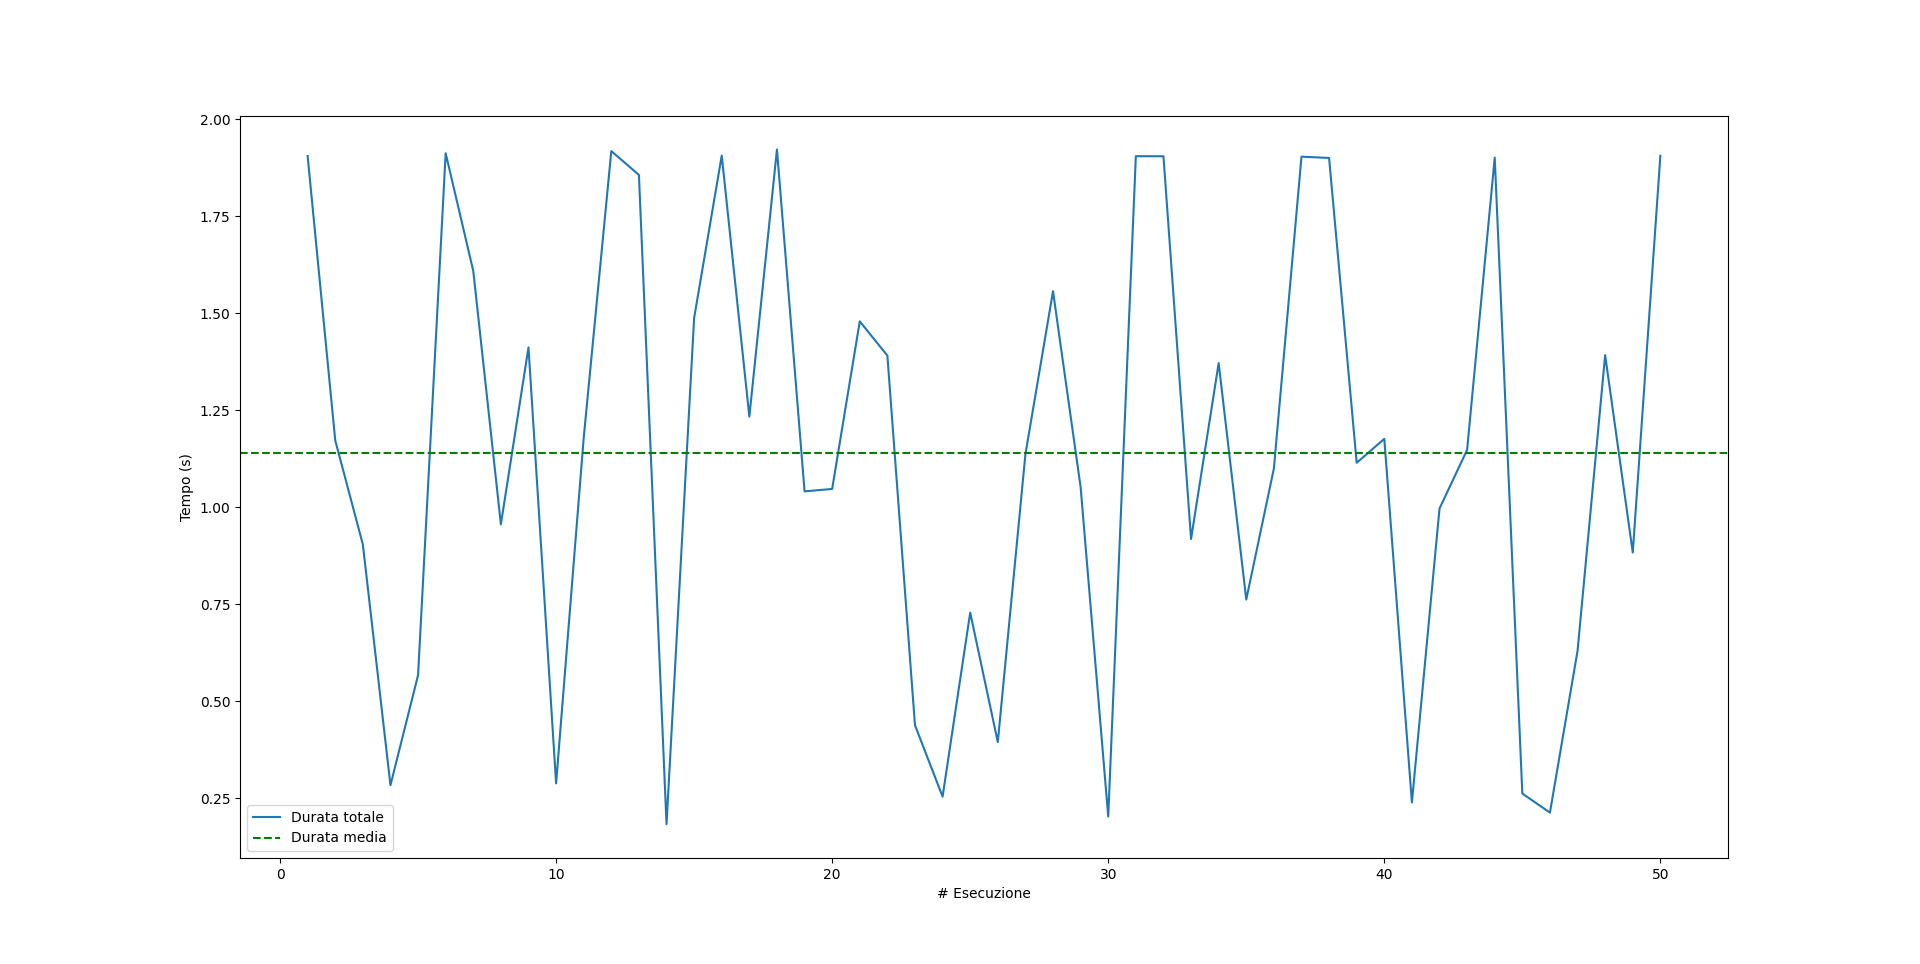
\includegraphics[scale=0.25]{results/esecuzioni}
\end{center}

Di seguito, alcuni risultati presi a campione.

\pagebreak{}

\begin{center}
	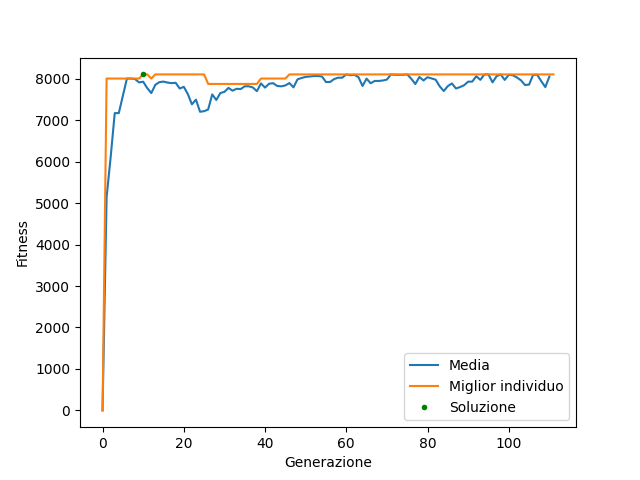
\includegraphics[scale=0.25]{results/0}
	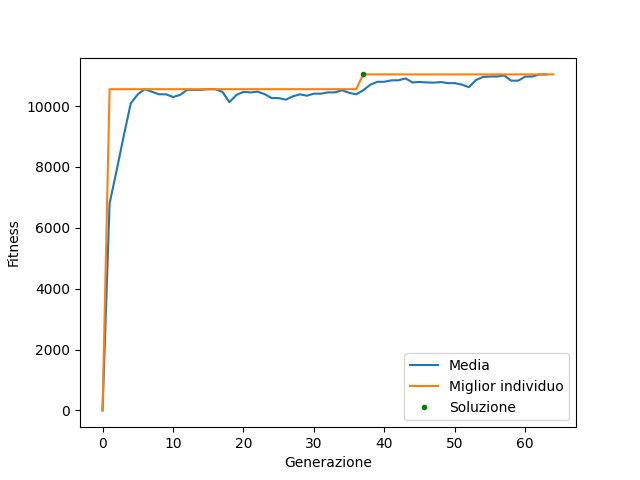
\includegraphics[scale=0.25]{results/1}
	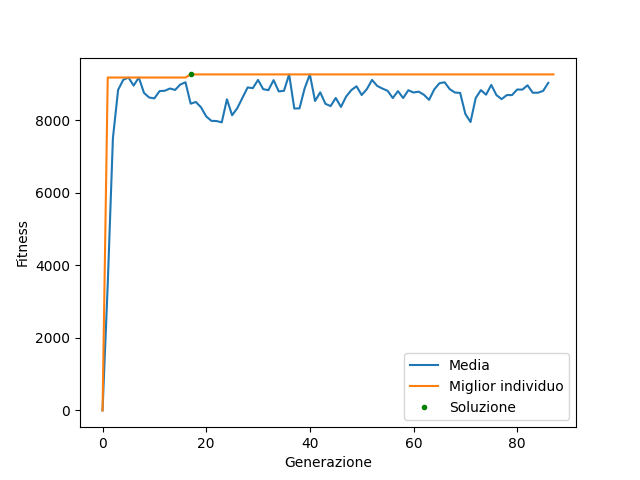
\includegraphics[scale=0.25]{results/2}
	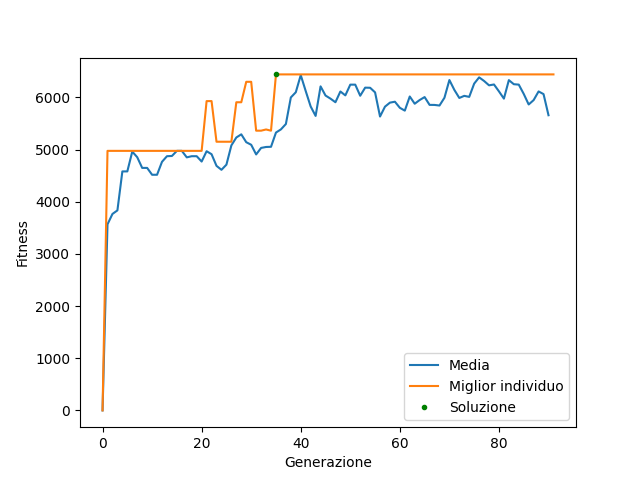
\includegraphics[scale=0.25]{results/3}
	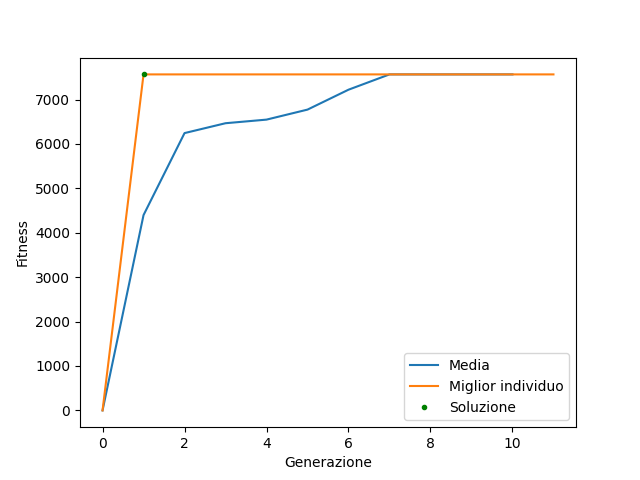
\includegraphics[scale=0.25]{results/4}
	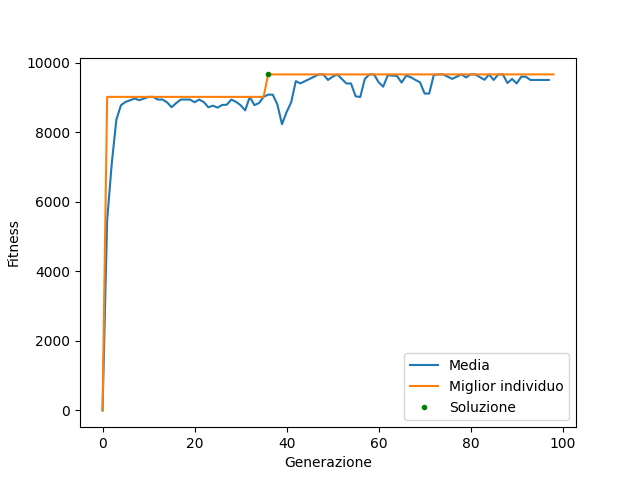
\includegraphics[scale=0.25]{results/5}
	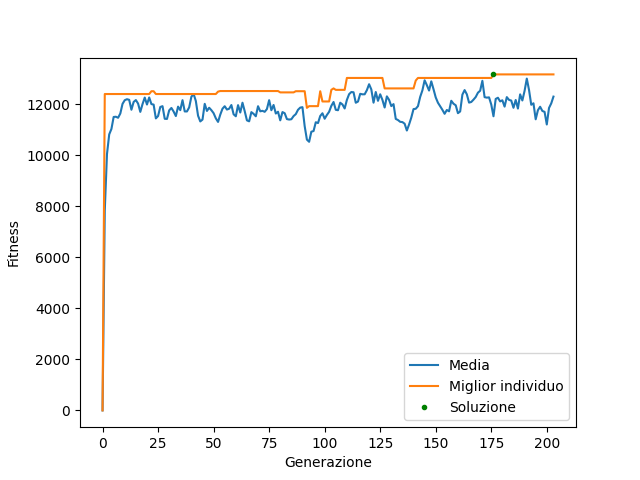
\includegraphics[scale=0.25]{results/6}
	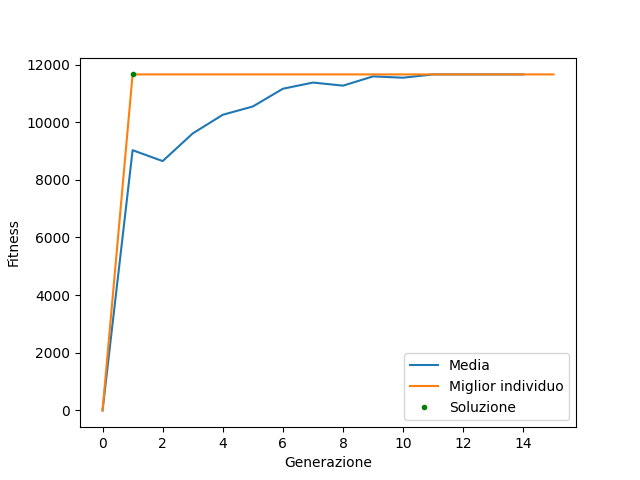
\includegraphics[scale=0.25]{results/7}
	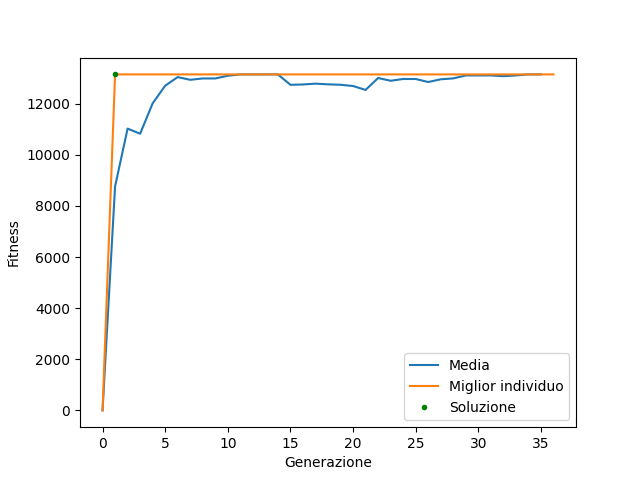
\includegraphics[scale=0.25]{results/8}
	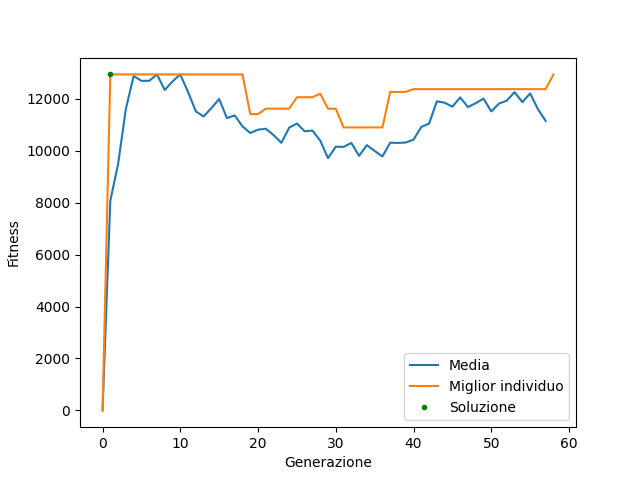
\includegraphics[scale=0.25]{results/9}
	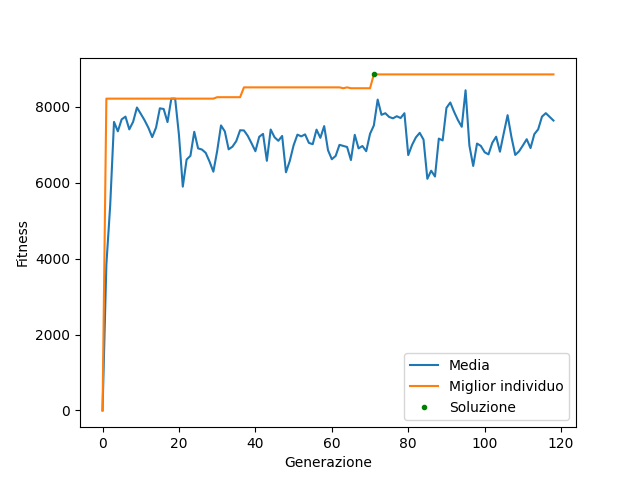
\includegraphics[scale=0.25]{results/10}
	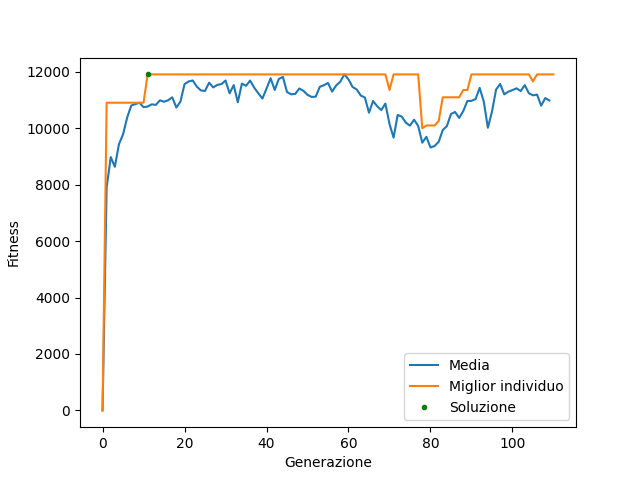
\includegraphics[scale=0.25]{results/11}
	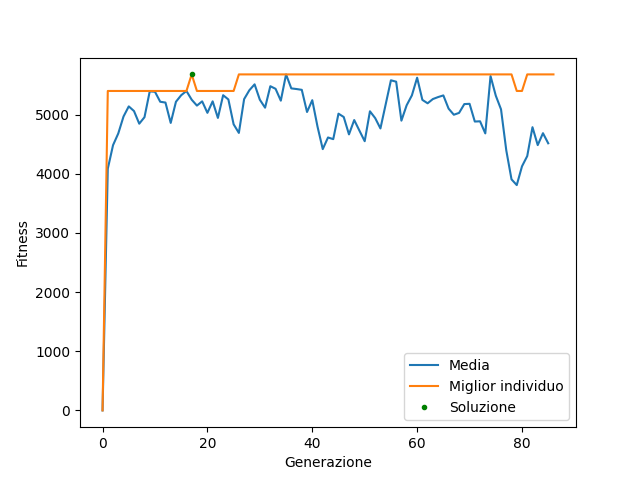
\includegraphics[scale=0.25]{results/12}
	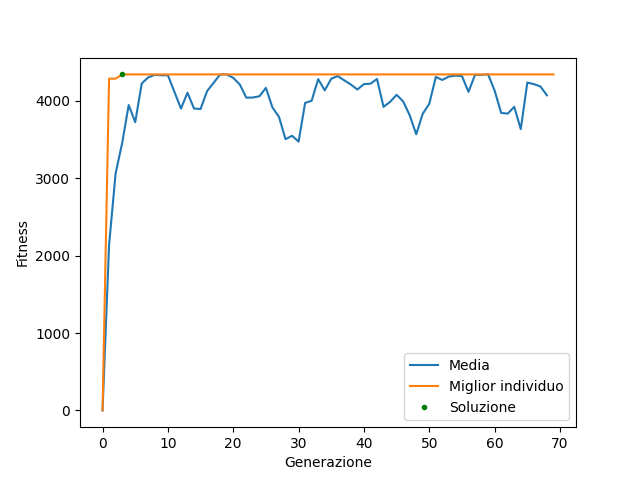
\includegraphics[scale=0.25]{results/13}
	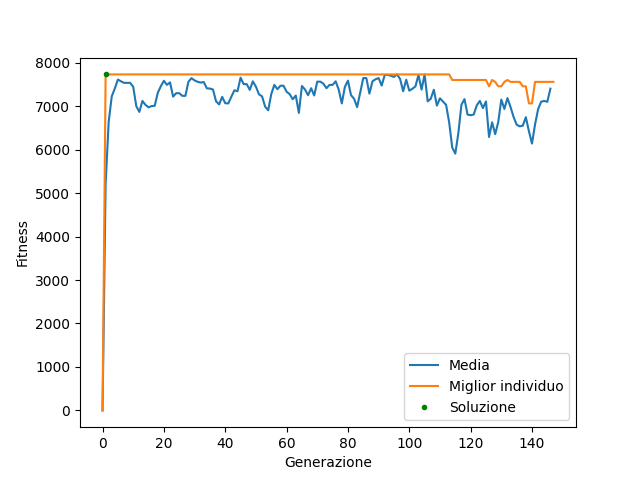
\includegraphics[scale=0.25]{results/14}
	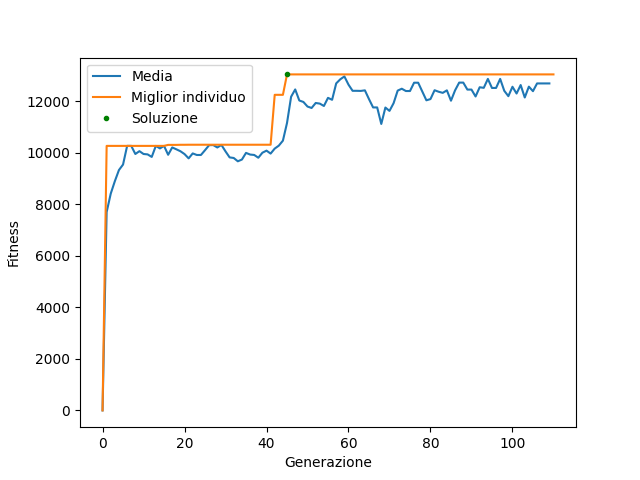
\includegraphics[scale=0.25]{results/15}
	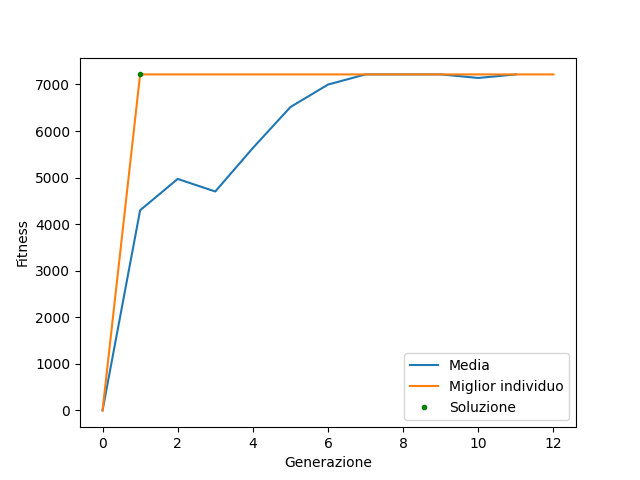
\includegraphics[scale=0.25]{results/16}
	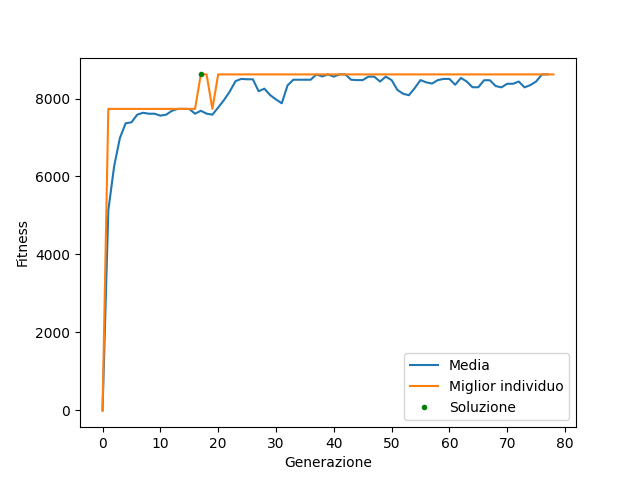
\includegraphics[scale=0.25]{results/17}
	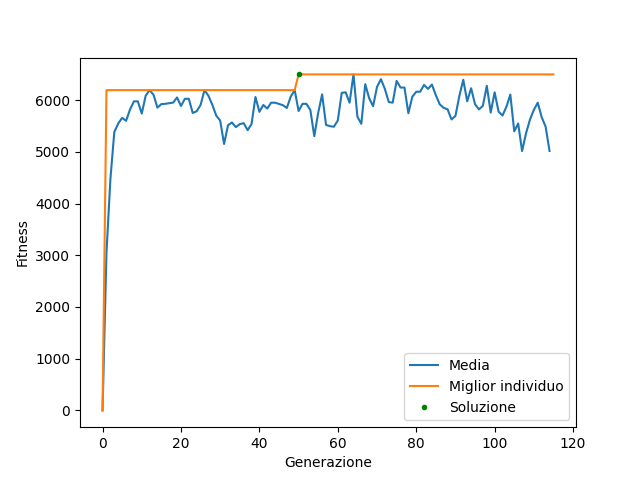
\includegraphics[scale=0.25]{results/18}
	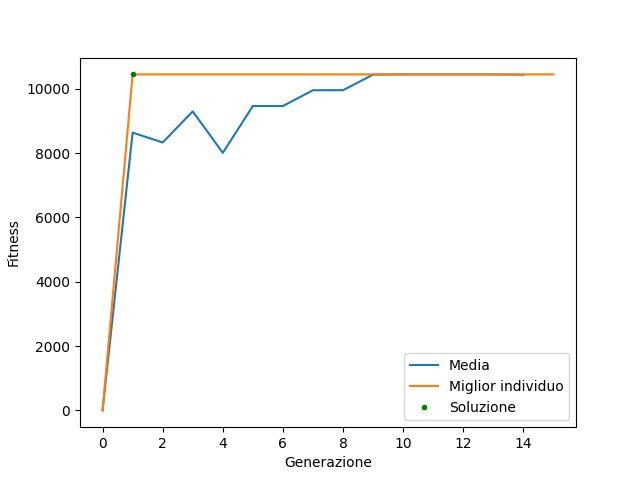
\includegraphics[scale=0.25]{results/19}
	
\end{center}

\pagebreak{}

\subsection{Considerazioni finali}

Seppur fornisca un'ottima approssimazione, l'algoritmo è decisamente migliorabile sotto diversi aspetti: in particolare, \textbf{la presenza di dati veritieri consentirebbe lo studio più approfondito} di eventuali problematiche non riscontrate con un dataset artificiale.

Infine, si potrebbe \textbf{considerare l'utilizzo di strutture dati create su misura, da sostituire ai K-D Tree}, per una più rapida e accurata individuazione delle strutture adiacenti.

\pagebreak{}
\section{Glossario}

\begin{itemize}
   \item \textbf{Problema di ottimizzazione}: problema il cui obiettivo è quello di ricercare il miglior valore possibile per una funzione obiettivo, soggetta a vincoli.
   \item \textbf{Algoritmo genetico}: problema di ottimizzazione che simula il processo evolutivo al fine di trovare soluzioni ottimali a problemi complessi.I suoi individui, ovvero la popolazione iniziale, attraverso operazioni di selezione, incrocio e mutazione, genereranno individui evoluti, che saranno sempre più vicini alla soluzione ottima.
   \item \textbf{Python}: linguaggio di programmazione ad alto livello, che si presta ad un semplice utilizzo per via della vicinanza al linguaggio naturale.
   \item \textbf{Large Language Model}: modello di deep learning, addestrato su grandi quantitativi di dati testuali, con l'obiettivo di apprendere e generare linguaggio naturale.
   \item \textbf{K-D Tree}: struttura dati gerarchica per organizzare punti in uno spazio k-dimensionale euclideo. A ogni livello dell'albero, lo spazio viene suddiviso alternando sistematicamente le $k$ dimensioni. Questi alberi sono utilizzati per l'organizzazione e la ricerca di dati multidimensionali. Sebbene le coordinate geografiche non rappresentino uno spazio euclideo, per distanze relativamente brevi sulla superficie terrestre gli effetti della curvatura possono essere trascurati, approssimando sufficientemente bene le distanze calcolate con le coordinate geografiche a quelle di uno spazio euclideo bidimensionale.
   \item \textbf{Funzione di fitness}: funzione di valutazione dei dati o di adattamento della soluzione candidata al problema in via di risoluzione. Essa assegna un punteggio ad ogni individuo della popolazione scelta, in base al livello di soddisfazione dell'obiettivo. Infatti, più alto è il punteggio di fitness di una soluzione, maggiore è la probabilità che essa venga selezionata e utilizzata per generare nuove soluzioni che si avvicineranno sempre di più alla soluzione ottimale.
   \item \textbf{Memoizzazione}: tecnica che consiste nel salvataggio in memoria dei valori restituiti da una funzione, in maniera tale da ricavarli facilmente per riutilizzi successivi, evitando di ricalcolare i risultati. 
\end{itemize}

\end{document}
